\documentclass[italian]{beamer}
%%%%
%%%%
\usecolortheme{lily}
\usetheme{AnnArbor}
%footline:
\setbeamertemplate{navigation symbols}{\insertframenumber}
\usepackage{pstricks}
\usepackage[tight,nice]{units}
\usepackage[]{url}
\usepackage{babel}
\usepackage[]{graphicx}
\usepackage[utf8x]{inputenc}
\usepackage[T1]{fontenc}
\usepackage{ae,aecompl}
\usepackage{nicefrac}
\include{pst-plot}
\include{pst-3d}
\newtheorem{definizione}{Definizione}
\frenchspacing
\pagestyle{empty}
\title{Discriminazione dei muoni da decadimenti di B e D}
\author{Matteo Abis \\
\url{matteo@latinblog.org}}
\institute{Università degli Studi di Padova\\
Scuola Galileiana di Studi Superiori}
\date{\today}
\begin{document}
\begin{frame}
    \titlepage
\end{frame}

\begin{frame}
    {Obiettivi dello studio}
    rivelatore CMS:\\
    discriminare tra mesoni B e mesoni D in decadimenti\\
    \begin{center}
        $B \to \mu X$\\
        $D \to \mu X$
    \end{center}
    attraverso le diverse distribuzioni del parametro d'impatto.
\end{frame}

\begin{frame}
    \begin{figure}[h]
        \begin{center}
            \includegraphics[width=\textwidth]{cms1.eps}
        \end{center}
    \end{figure}
\end{frame}

\begin{frame}{Struttura di CMS}
    \begin{description}
        \item[Tracker] cilindri concentrici di sensori al silicio. Misura
            l'impulso delle particelle cariche
        \item[Calorimetri] misurano l'energia di elettroni e fotoni (ECAL) o
            di altri adroni (HCAL) 
        \item[Rivelatori $\mu$] camere a deriva, solo i muoni sono abbastanza
            penetranti da raggiungerle.
    \end{description}
    \begin{figure}[h]
        \begin{center}
            \includegraphics[height=0.5\textheight]{cms_track.eps}
        \end{center}
    \end{figure}
\end{frame}

\begin{frame}{Sistema di riferimento di CMS}
    \begin{itemize}
        \item pseudorapidità $\eta = -\log \tan
            \nicefrac{\theta}{2}$
        \item $\eta$ ha lo stesso segno di $z$ e va da $-\infty$ a
            $+\infty$
    \end{itemize}
\begin{figure}[h]
    \begin{center}
        \psset{unit=1.15,viewpoint=2 1.5 1}
        \begin{pspicture}(0,0)(2.5,2.5)
            %xz plane
            \psset{arrows=->}
            \ThreeDput[normal=0 0 1]{
            \psline[linewidth=1pt]{}(0,0)(2, 1.154)
            \psarc{->}{1}{0}{30}
            \rput[l]{120}(1.35, 0.30){$\theta$}
            }      

            %zy plane
            \ThreeDput[normal=0 1 0]{
            \psline(0,0)(0,3)
            \psline(0,0)(-3,0)\uput[0](-3.5,0){$z$}
            \uput[0](-4.5,0.5){\small{direz. del fascio}}
            }      

            %xy plane
            \ThreeDput[normal=1 0 0]{
            \psline(0,0)(3,0)\uput[0](3,0){$x$}
            \uput[0](2.5,0.5){\small{centro di LHC}}
            \uput[0](0,3){$y$}
            \psline[linewidth=1pt]{}(0,0)(2,1.154)
            \psarc{->}{1}{0}{30}
            \uput[0](1.05,0.40){$\phi$}
            }      
        \end{pspicture}
    \end{center}
\end{figure}
\end{frame}

\begin{frame}{Dati Monte Carlo}{un milione di eventi $pp \to \mu X$}
Selezione delle tracce ricostruite:
\begin{itemize}
    \item identificazione dei muoni:
        \begin{itemize}
            \item hit nell'ultima camera a $\mu$
            \item almeno due segmenti compatibili nelle camere a $\mu$
            \item segmenti nel \emph{tracker} ben accoppiati con i segmenti
                nelle camere a $\mu$
        \end{itemize}
    \item $p_t > \unit[3]{GeV/c}$, trigger e campo magnetico di CMS
    \item $|\eta| < 2.5$
\end{itemize}
    \begin{figure}[h]
        \begin{center}
            \includegraphics[height=0.4\textheight]{cms_track.eps}
        \end{center}
    \end{figure}
\end{frame}
    
\begin{frame}{Associazione tracce ricostruite $\to$ particelle generate}
    Non c'è codice appositamente sviluppato al CERN
\begin{itemize}
    \item minima distanza nello spazio $(\eta, \phi)$. $\Delta R =
        \sqrt{\Delta \eta^{2} + \Delta \phi^{2}}$
    \item ulteriore taglio delle coppie con $\Delta R < 0.1$ o $\Delta p_t /
        p_t < 0.1$
\end{itemize}
\begin{figure}[h]
    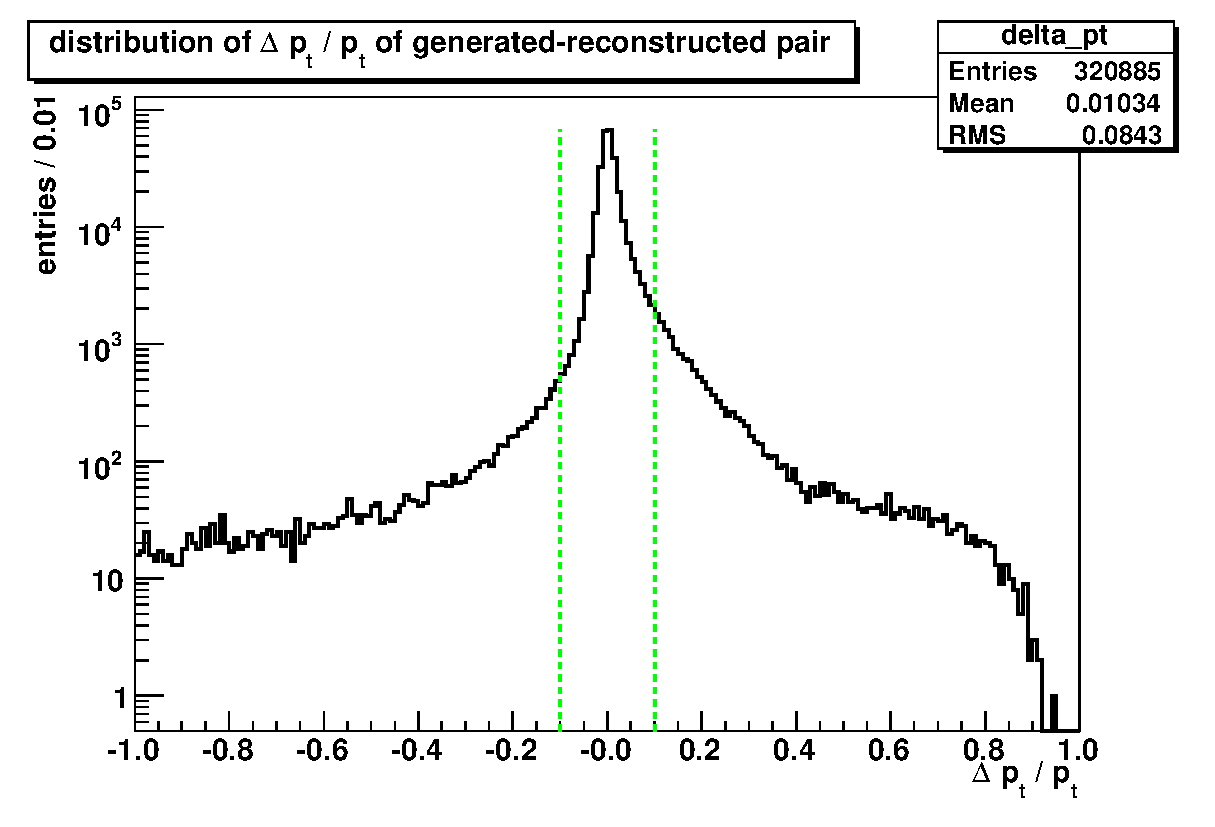
\includegraphics[width=0.5\textwidth]{crea_istogrammi/delta_pt.eps}
    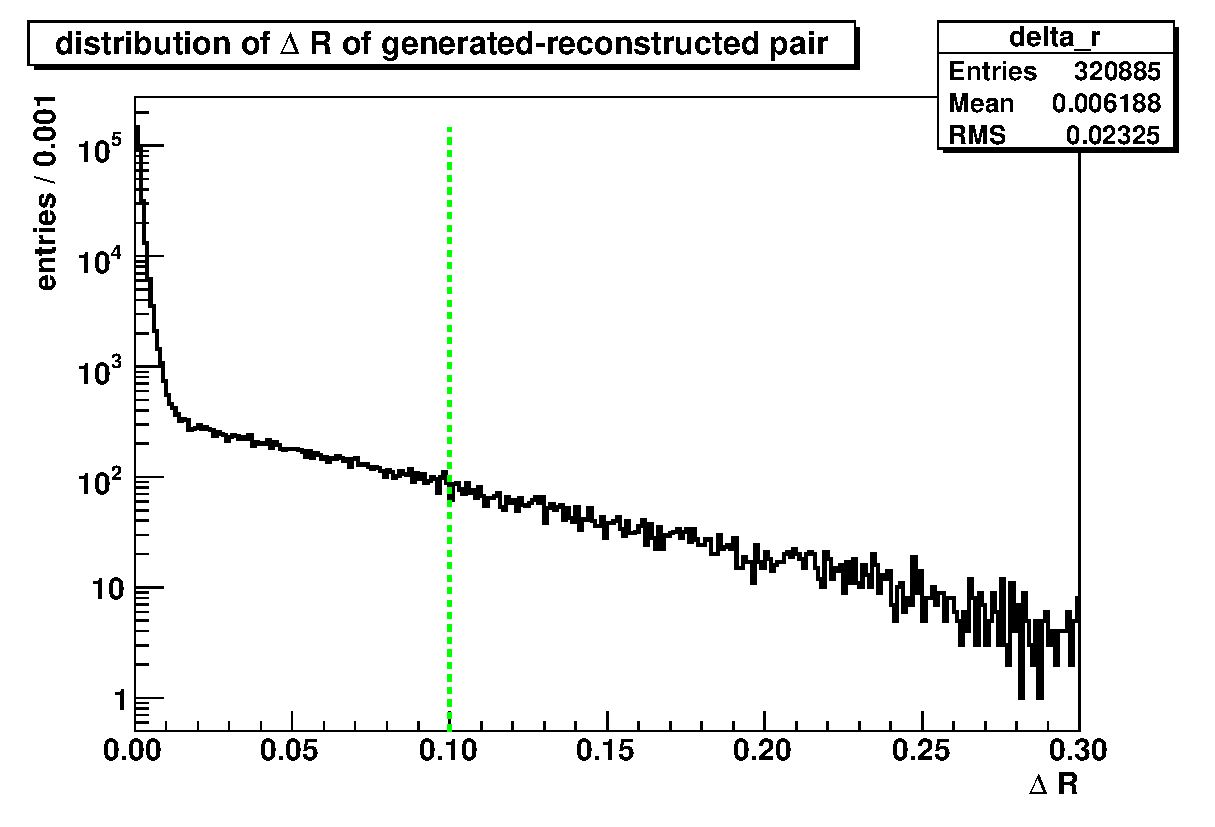
\includegraphics[width=0.5\textwidth]{crea_istogrammi/delta_r.eps}
\end{figure}
\end{frame}

\begin{frame}{Parametro d'impatto $d$}
    \begin{definizione}
       la minima distanza sul piano trasverso fra la traccia estrapolata
       e il punto dell'interazione tra i fasci di protoni.
    \end{definizione}

\begin{itemize}
    \item $\tau_D = \unit[0.4]{ps}$ e $\tau_B = \unit[1.6]{ps}$ $\to$
        diverse distribuzioni in $d$
    \item parametro d'impatto $d$ $\to$ discriminare B e D
\end{itemize}
\begin{figure}[h]
    \psset{unit=0.8}
    \begin{pspicture*}(-1,-1)(4,4)
        \psaxes*[labels=none,ticks=none,linewidth=.6pt]{->}(0,0)(-1,-1)(4,4)      
        \psellipticarc[]{<-}(5,2)(3.5,3.5){150}{180}
        \psellipticarc[linestyle=dashed,dash=0.2 0.15]{}(5,2)(3.5,3.5){180}{240}
        \psline[linewidth=0.8pt,linestyle=dashed,dash=0.1 0.1]{}(0,0)(1.75, 0.7)
        \uput*[30](0.58, 0.25){$d$}
        \uput*[225](0, 0){$PV$}
        \rput[r]{*0}(-0.2, 3.8){$y$}
        \rput[l]{*0}(2.1, 3){traccia}
        \rput[r]{*0}(1.4, 2){$DV$}
        \rput[t]{*0}(3.8, -0.2){$x$}
    \end{pspicture*}
\end{figure}
\end{frame}

\begin{frame}{Distribuzioni in $d$}
Dipendenze analizzate:
\begin{itemize}
    \item \emph{global track} e \emph{inner track}
    \item $p_t$ minimo
    \item luminosità integrata (numero di eventi)
\end{itemize}
\begin{figure}[h]
    \includegraphics[width=0.5\textwidth]{crea_istogrammi/d_lin_inner.eps}
    \includegraphics[width=0.5\textwidth]{crea_istogrammi/d_lin_global.eps}
\end{figure}
\end{frame}

\begin{frame}{Test di Kolmogorov-Smirnov}
    \begin{block}{}
        probabilità che due campioni provengano dalla stessa popolazione
    \end{block}
\begin{itemize}
    \item distribuzioni cumulative
    \item massima distanza
    \item probabilità
\end{itemize}
\end{frame}

\begin{frame}
    {In funzione del numero di eventi}{selezione $p_t > \unit[3]{GeV/c}$}
    $5\sigma$ $\to$ $\unit[7\cdot 10^{-3}]{pb^{-1}}$ ($\approx$
    \unit[250 000]{$\mu$}) 
\begin{figure}[h]
    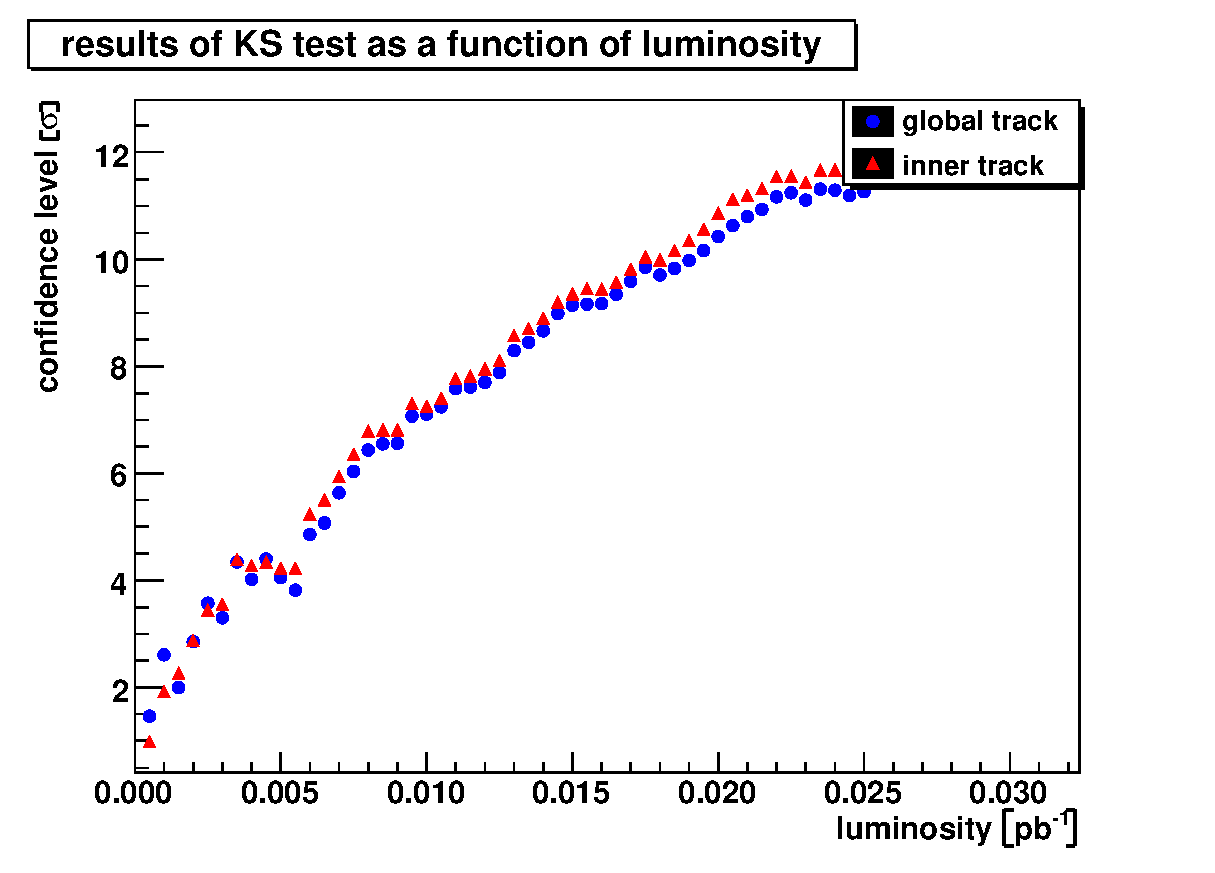
\includegraphics[width=0.7\textwidth]{crea_istogrammi/lum_1.eps}
\end{figure}
\end{frame}

\begin{frame}{In funzione di $p_t$}
    il livello di confidenza scende perch\'e diminuisce la significanza
    statistica del campione.
\begin{figure}[h]
    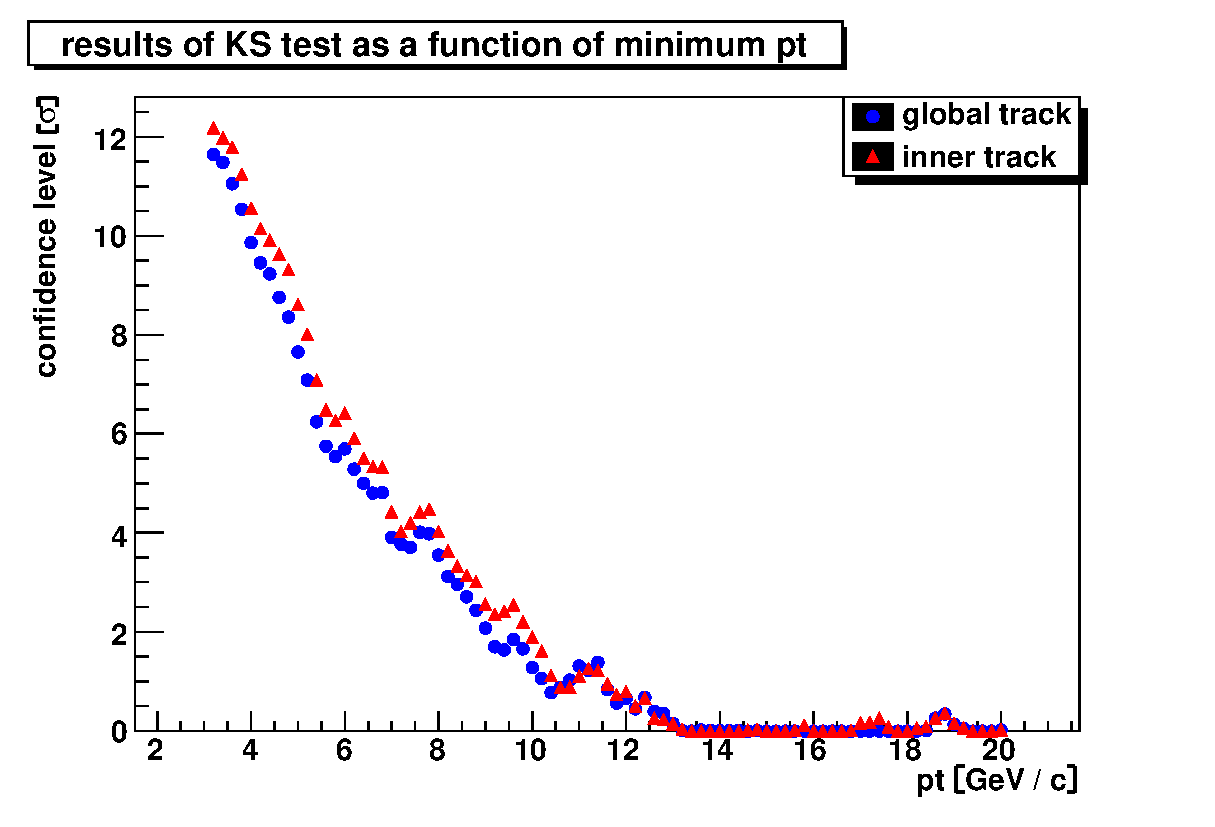
\includegraphics[width=0.7\textwidth]{crea_istogrammi/pt_1.eps}
\end{figure}
\end{frame}

\begin{frame}{Pseudo-esperimenti}{eliminare la dipendenza dal numero di
    eventi}
    \begin{itemize}
        \item<1-> distribuzione $d$ dei $\mu$ che superano la selezione richiesto
        \item<2-> due istogrammi da 10000 GetRandom dalle distribuzioni
        \item<3-> test di Kolmogorov
        \item<3-> si ripete 100 volte, media e RMS sul grafico 
    \end{itemize}
\begin{figure}[h]
    \includegraphics<4->[height=0.6\textheight]{crea_istogrammi/pseudo_pt_1.eps}
\end{figure}
\end{frame}

\begin{frame}{Conclusioni} 
    \begin{itemize}
        \item luminosità integrata $\to 5\sigma$: $\unit[7\cdot
            10^{-3}]{pb^{-1}} \approx$ 1--12 giorni di
            LHC\footnote{Stima della luminosità istantanea tra
            $\unit[10^{30}]{cm^{-2}s^{-1}}$ e $\unit[10^{31}]{cm^{-2}s^{-1}}$}. 
        \item selezione $p_t$ più alto non sembra influenzare la discriminazione
        \item \emph{inner track} discrimina meglio di \emph{global track}
    \end{itemize}
\end{frame}

\end{document}
